\documentclass{article}
\usepackage{graphicx}
\usepackage[margin=1.5cm]{geometry}
\usepackage{amsmath}

\begin{document}
\twocolumn

\title{Friday Warm Up: Unit 0, E-fields of Charge Distributions}
\author{Prof. Jordan C. Hanson}

\maketitle

\section{Memory Bank}

\begin{itemize}
\item $\vec{F}_{\rm C} = k q_1 q_2 / r^2 ~~\hat{r}$ ... Coulomb force.
\item $k = 8.988 \times 10^{9}$ N C$^{-2}$ m$^{2}$ ... The constant of proportionality in Coulomb force.
\item $\vec{F} = q\vec{E}$ ... Definition of an electric field.
\item $1e = 1.602 \times 10^{-19}$ Coulombs ... Fundamental unit of charge.
\item $\vec{E} = k q/r^2 ~~\hat{r}$ ... Electric field of a point charge.
\end{itemize}

\begin{figure}
\centering
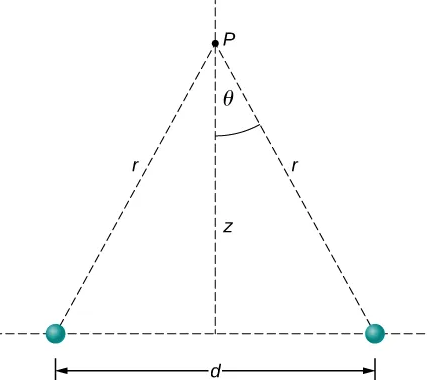
\includegraphics[width=0.33\textwidth]{figures/dipole.png}
\caption{\label{fig:1} Two charges separated by a distance $d$.}
\end{figure}

\section{Electrostatics I: Fields of Charge Distributions}

\begin{enumerate}
\item (a) Consider Fig. \ref{fig:1}.  If the spheres represent positive charges $q$, what is the $\vec{E}$-field at the origin? (b) What is the direction of the $\vec{E}$-field at point $P$?  (c) Derive an expression for the $\vec{E}$-field at point $P$. \\ \vspace{4cm}
\item Suppose four charges $q$ form a square of side length $a$, centered at the origin.  (a) What is the net $\vec{E}$-field at the origin? (b) Suppose the charge at $(d,d)$ is removed.  What is the net $\vec{E}$-field? (c) If a free charge $q_f$ and mass $m$ is released from $(d,d)$, and the other charges are held in place, what is the acceleration vector of $q_f$? (d) What is the kinetic energy of $q_f$ at time $t$? \\ \vspace{4cm}
\item A proton enters the uniform electric field produced by the two charged plates shown below. The magnitude of the electric field is $4 \times 10^5$ N C$^{-1}$, and the speed of the proton when it enters is $1.5 \times 10^7$ m s$^{-1}$.  By what distance $d$ has the proton been deflected downward when it leaves the plates?
\end{enumerate}

\begin{figure}
\centering
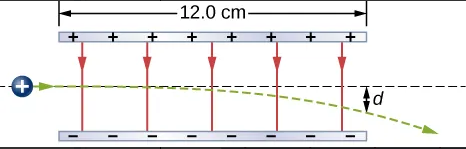
\includegraphics[width=0.45\textwidth]{figures/deflect.png}
\caption{\label{fig:2} A device for deflecting charged particle trajectories, or part of a mass spectrometer.}
\end{figure}

\end{document}
